\section{Remote Photoplethysmography}

To measure the heart beat and the heart beat variability a technology called remote Photoplethysmography can be employed \cite{verkruysse2008remote}.

First, the theoretical foundations are explained, followed by a discussion on the optimal regions of interest within the facial area. Based on these regions, various approaches for detecting and tracking the ROI are presented. Furthermore, the chapter examines traditional methods of feature extraction before discussing modern artificial intelligence-based paradigms.

\subsection{Theoretical Foundations}
The foundational work for modern remote photoplethysmography (rPPG) was made by Verkruysse et al. (2008), who demonstrated that the heart beat could be monitored using a standard digital camera. This relies on the fact that hemoglobin absords light differently than the neighboring body tissue. As the blood volume changes in the body with every heartbeat, the intensity of the reflected light varies. Their research identified that the green color channel contains the strongest information regarding the heart beat (Figure \ref{fig:blood_frequencies}). Despite the successful proof-of-concept, two challenges were highlighted: Motion artifcats caused by movement and  noise due to the camera's sensor \cite{verkruysse2008remote}.

%  hier noch auf das Beer-Lambert Law eingehen
\begin{figure}[!ht]
    \centering
    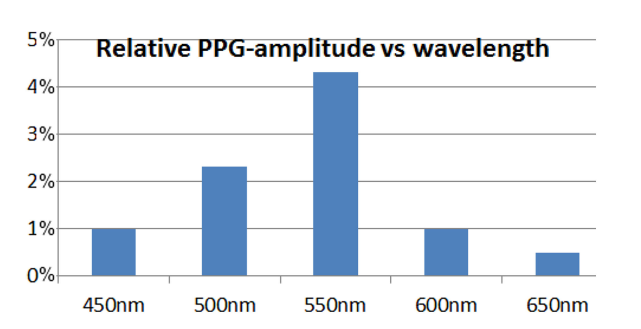
\includegraphics[width=0.9\columnwidth]{./chapters/pictures/blood_frequencies.png}
    \caption{Spectral sensitivity of the PPG signal. Green light exhibits the highest amplitude, making it the most reliable channel for non-contact heart rate monitoring. \cite{dehaan2013chrom}}
    \label{fig:blood_frequencies}
\end{figure}


\subsection{Face Detection and region of interest selection}

The selection of the right region of interest for rPPG measurements is critical for the suppression of motion and illumination artifacts. Previous approaches often utilized the entire face as a global ROI for signal extraction. However, Lempe et al. (2013) demonstrated that the signal quality varies substantially across different facial areas \cite{lempe2013roi}.

To quantify this, they implemented a grid layout over the face and calculated the local signal-to-noise ratio for each segment. Through this spatial analysis, the cheek regions were identified as the most promising areas for pulse extraction (Figure \ref{fig:roi}) \cite{lempe2013roi}.

A significant practical advantage of the cheeks is that they are rarely covered by clothing or facial hair, which supports a more stable measurement compared to a global face ROI. These findings highlight a significant technical challenge. The requirement for advanced segmentation and tracking algorithms that can reliably detect and follow the cheek area, even during head movements, to ensure a consistent and high-quality pulse signal \cite{lempe2013roi}.

\begin{figure}[!ht]
    \centering
    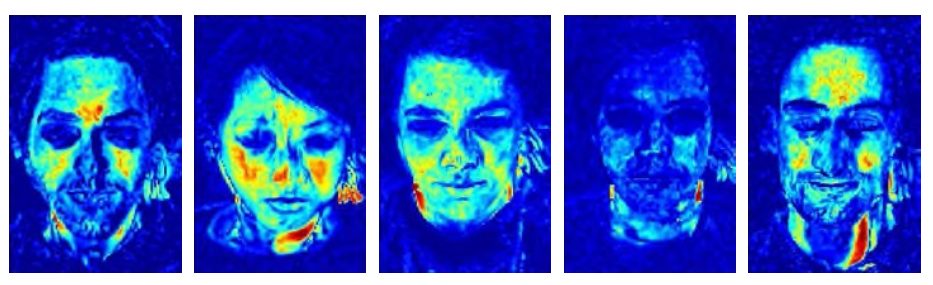
\includegraphics[width=0.9\columnwidth]{./chapters/pictures/ROI.png}
    \caption{The quality of the rPPG signal in the face. Blue shows low activity and red hight activity \cite{lempe2013roi}}
    \label{fig:roi}
\end{figure}

\subsubsection{Landmark Tracking}


Lempe et al. (2013) identified the optimal regions for extraction. The challenge is to keep these region of interests stable and to handle noise due to motion and light changes. Especially in the use case of human-computer interaction, brightness changes lead to severe fluctuations of pixel values in the face, examples include watching a movie or gaming. Li et al. (2014) propose a framework to solve these issues. First of all, the viola-jones detector is used to get a rough estimation of the face location. Then, 66 facial landmarks are placed, and based on these landmarks, a precise mask for the region of interest is generated.To maintain a stable measurement, the Kanade-Lucas-Tomasi (KLT) feature tracker is employed. KLT points are used to continuously track the face, ensuring it is also tracked when moved. A second important step is the correction of brightness changes. It is assumed that these changes are not only visible in the face but also in the background. The average brightness changes in both the background and the face are measured, and a normalized least mean squares filter is used to find the optimal coefficient to subtract background noise from the facial area. Furthermore, non-rigid movement like smiling or speaking induces changes in the skin which cannot be compensated through tracking alone. Consequently, the measurements are split into small segments, and those with a high standard deviation are discarded. This framework was tested with the sophisticated MAHNOB-HCI database and reached a low error score of 6.87\% with 527 users. Despite these achievements, there are still quite a few problems; for instance, large head movements lead to a significant loss of KLT tracker points, which results in an unstable localization of the ROI \cite{li2014remote}.

\subsubsection{High-Density 3d Face Mesh}

A limitation of traditional landmark-based tracking systems is that they have a reduced robustness against head rotations or non-rigid deformations. To overcome these hurdles, there have been approaches to use artificial intelligence to reach a higher resolution. The previous model by Li et al. used 66 vertices, while this new approach by Kartynnik et al. (2019) uses a dense 3D mesh consisting of 468 vertices. This model creates a 3D mesh of the face, meaning it can estimate the depth of each point even from a normal 2D camera (Figure \ref{fig:facemesh}). Depending on the hardware, it can deliver 100 to 1000+ FPS \cite{kartynnik2019real}.

Different models that also use many vertices often use standard methods based on averaging effects. They don't work well when there are small inaccuracies, like the closing of one eye. Due to the architecture of the neural network developed by Kartynnik and his team, it is possible to use it in real-time. It has been trained on a dataset of around 30,000 images. It has been tested that it has the same accuracy as human experts that model the face \cite{kartynnik2019real}.

\begin{figure}[!ht]
    \centering
    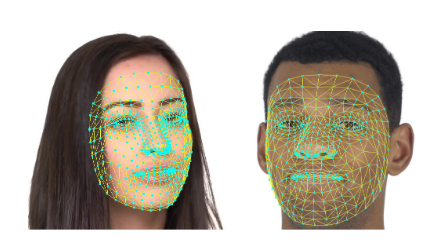
\includegraphics[width=0.9\columnwidth]{./chapters/pictures/face_mesh.png}
    \caption{Example of a face mesh calculating with an artificial intelligence model \cite{kartynnik2019real}}
    \label{fig:facemesh}
\end{figure}

\subsection{Traditional Frameworks for signal extraction}

Traditional rPPG frameworks typically follow a multi-stage process. First, the face is detected and tracked, often using the Viola-Jones algorithm or similar cascade classifiers to define a region of interest. Then methods such as Principal component Analysis (PCA) or Independet Component Analysis (ICA) are employed to isolate the pulse signal from the green color channel. While effective if the person remains still, these approaches struggle with motion artifacts, as they require quite a few seconds of stable data to compute the signal components \cite{Debnath25}.

\subsubsection{Blind Source Separation}

Poh et al. (2010) introduced blind source separation (BSS) to rPPG. Their framework assumes that the recorded RGB channels do not only contain the pulse information but also significant noise in the form of light changes and movement. The challenge is that this noise has to be separated from the real physiological information. Mathematically speaking, the resulting color channels are treated as a linear mixture \cite{poh2010non}:

$$x(t) = As(t)$$

The goal is to find a demixing matrix $W$, so that the original source signals $\hat{s}(t) = Wx(t)$ can be calculated. To find $W$, it is important to search for statistical independence between the sources. For that, the JADE algorithm (Joint Approximate Diagonalization of Eigenmatrices) is used. Unlike deterministic methods, JADE is an iterative process that tries out different combinations to maximize non-Gaussianity, which results in a higher computational load and increased latency (Figure \ref{fig:color_channels}) \cite{poh2010non}.

\begin{figure}[!ht]
    \centering
    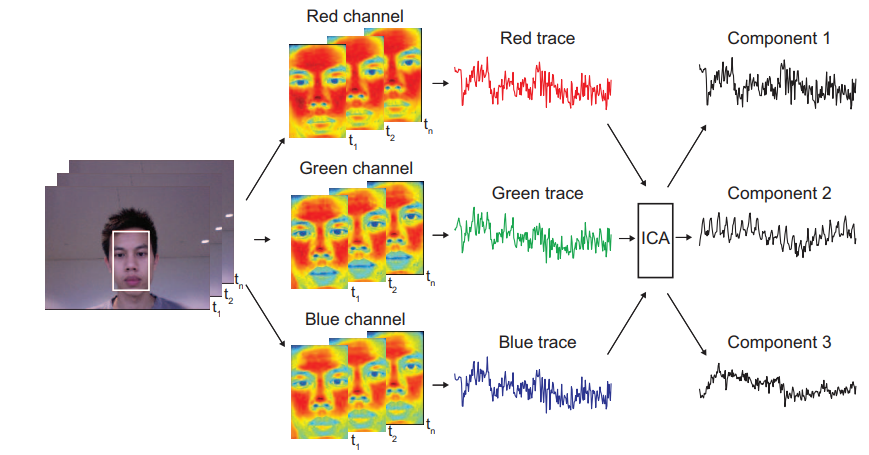
\includegraphics[width=0.9\columnwidth]{./chapters/pictures/color_channels.png}
    \caption{Seperation of color channels \cite{poh2010non}}
    \label{fig:color_channels}
\end{figure}


For the initial localization, the viola-Jones algorithm is used to detect the face. In this specific setup, only 60\% of the bounding box width is used as the Region of Interest. The raw signals from this ROI are then spatially averaged and normalized using Zero-Mean and Unit-Variance to balance different channel intensities \cite{poh2010non}.

After the independent components are recovered, the pulse is extracted by using the fast fourier transform. An operational range from [0.75 - 4.0] Hz is allowed, because this corresponds to 45 - 240 BPM, the range a human pulse usually lies in. Additionally, a temporal consistency threshold is implemented.A jump of only 12 BPM is allowed between consecutive measurements that are taken one second apart. Anything different is rejected as noise or an artifact. The highest power peak within the frequency spectrum is chosen as the final heart rate \cite{poh2010non}.

To compare the accuracy of this methodology to a gold standard Bland-Altman plots are used. These plots show that ICA can significantly reduce the Root Mean Squared Error (RMSE) from 19 BPM to about 4.6 BPM even when the subject is moving \cite{poh2010non}.

However, there are physical limitations to consider. According to the Beer-Lambert Law, the way light travels through and is absorbed by blood vessels is technically non-linear. But for the sake of computation, ICA uses a linear approximation, which works well for short time windows. The system is also highly dependent on the ambient lumination. If it is too dark, the SNR drops too low for a reliable measurement \cite{poh2010non}.

Another risk is that the wrong component is picked. In this study, the second independent component is usually chosen as the pulse signal because hemoglobin absorptivity is highest in the green spectrum. However, this fixed selection could be wrong if the noise is too strong. Finally, it is noted that using simple webcams is much more cost-effective than using expensive thermal cameras, and the software-based approach even allows for the simultaneous detection of multiple people in one frame \cite{poh2010non}.

\subsection{The Chrominance-based Method}

Blind source separation (BSS) techniques provide a powerful mathematical tool for signal isolation. Nevertheless, these techniques face significant challenges in scenarios with substantial motion and light artifacts. To address these limitations, de Haan and Jeanne (2013) proposed a physics-based alternative known as the Chrominance-based method (CHROM). It effectively addresses the challenge of subject motion when calculating the heart rate, as periodic movements can render simple intensity-based selections useless. Furthermore, while many algorithms require long observation intervals to achieve sufficient frequency resolution, CHROM is designed to be highly efficient. Similarly to traditional methods like PCA or ICA, the CHROM algorithm utilizes the fact that blood absorbs a large percentage of green light. Additionally, it analyzes how light is reflected by human skin. According to the dichromatic reflection model, this reflection consists of a specular and a diffuse component (Figure \ref{fig:chrom_light}).According to the model of de Haan, a measured signal $C_i$ for every color channel can be written as \cite{dehaan2013chrom}:

$$C_i = I \cdot ( \rho C_{dc} + \rho C_i + s_i )$$

Here, $\rho C_{dc}$ represents the constant color of the skin, $\rho C_i$ the pulsating change due to blood flow and $s_i$ the specular reflection. Only the diffuse reflection enters the skin and carries the color of the blood. The specular reflection, however, does not enter the skin. It is reflected directly off the surface and thus contains no information about the blood. Since this specular part is an additive value, a simple division of color channels cannot cancel this effect. Therefore, CHROM uses a subtractive approach \cite{dehaan2013chrom}:
$$(R + noise) - (G + noise) = R - G$$

\begin{figure}[!ht]

    \centering

    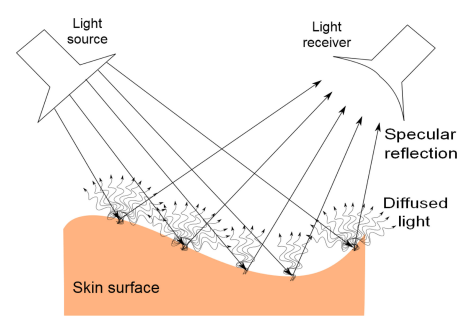
\includegraphics[width=0.9\columnwidth]{./chapters/pictures/chrom_light.png}

    \caption{The illustration depicts light reflection on the skin \cite{dehaan2013chrom}}

    \label{fig:chrom_light}

\end{figure}


Light intensity changes ($I$) and specular reflections ($s_i$) influence all color channels proportionally. Consequently, these noise vectors primarily move along a single axis in the color space. To reduce these effects, CHROM projects the normalized RGB signals onto a plane that runs perpendicular to the standard skin color vector. Based on empirical data from a diverse set of subjects, de Haan and Jeanne derived a standardized average vector for skin color: $[0.7682, 0.5121, 0.3841]$. By projecting the signals onto the orthogonal $X$ and $Y$ planes using this vector, the diffuse and specular light components cancel each other out. The resulting signals $X_s$ and $Y_s$ are thus largely free of luminance changes \cite{dehaan2013chrom}:

$$X_s = 3R_n - 2G_n$$$$Y_s = 1.5R_n + G_n - 1.5B_n$$

These two orthogonal planes can be comined with a factor $\alpha$. This represents the light absorption of hemoglobin \cite{dehaan2013chrom}:

$$S = X_s - \alpha \cdot Y_s \quad where \quad \alpha = \frac{\sigma(X_s)}{\sigma(Y_s)}$$

Even after projection, the signal $S$ may contain a slow drift caused by respiration or minor posture changes. To isolate the cardiac signal, a Bandpass Filter is applied, typically tuned to a range of 0.7 Hz to 4.0 Hz (42 to 240 BPM). Finally, a Fast Fourier Transform (FFT) is performed on the filtered signal to identify the dominant peak in the power spectrum. For instance, a peak at 1.2 Hz corresponds to \cite{dehaan2013chrom}:


$$1.2 Hz \times 60 seconds = 72 BPM$$

One of the most significant advantages of CHROM is its temporal efficiency. While traditional BSS methods (Blind Source Separation) like ICA or PCA often require up to 30 seconds of data to stabilize, CHROM utilizes an Overlap-Add (WOLA) procedure. By using overlapping windows of only 1.6 seconds, the system provides a continuous, near-instantaneous pulse estimate \cite{dehaan2013chrom}.

In comparative studies, the robustness of CHROM is evident. CHROM has a high stationary accuracy and predictes the correct pulse with a 98\% accuracy. It has a 92\% correlation with the medical-grade contact sensor. Furthermore, it is resilient against motion. Under heavy motion, e.g., on a fitness stepper, it maintains a 48\% success rate. ICA and PCA fail significantly, and only reach 4\% and 11\%. Moreover, CHROM can also process different skin tones. Darker skin tones naturally lower the Signal-to-Noise ratio because they absord more light. Chrom remains the most robust classical algorithm across all phenotypes \cite{dehaan2013chrom}.

\subsubsection{Modern Deep Learning Paradigms}

While physics-based methods like CHROM improved the handling of light and motion artificats, they are still based on fixed mathematical assumptions. To overcome these hurdles the field has increasingly shifted towards artificial intellligence models \cite{Debnath25}.

Following the initial proof-of-concept, a significant increase in rPPG research was observed, particularly after 2017. This trend is closely linked to the rapid improvements in artificial intelligence and deep learning. In 2025 82.05\% \cite{Debnath25} of papers about rPPG technology used an approach with artificial intelligence. A major problem is the availability of diverse, large-scale datasets. The available sets only have data of people from North America, Europe and China. This leads to a huge underrepresentation of various age groups and diverse skin pigmentations \cite{Debnath25}.

With the rapid advancement in artificial intelligence, modern rPPG systems have shifted towards end-to-end models. These architectures can process raw data or image sequences to estimate heart rate directly, often without the need for manual face isolation or region of intrest  selection. There are three architectural paradigms: Convolutional Neural Networks (CNNs), Hybrid Neural Networks and Transformed-based architectures \cite{Debnath25}.

In modern rPPG systems, convolutional neural networks (CNNs) are the standard for processing image data. Their main task is to recognize the very subtle color changes in the skin pixels that happen during a cardiac cycle \cite{Debnath25}.

A big problem in this field, is that there aren't enough large and diverse datasets to train these models from scratch. Because of this, researchers often use transfer learning \cite{Debnath25}. The idea here is to take a model that was already trained on a different task, such as general face recognition. By freezing the first layers and only fine-tuning the last ones with rPPG-specific data, the model can use its existing knowledge of facial features. This approach makes it possible to get good results even with smaller datasets and saves a lot of training time \cite{pan2009survey}.
Furthermore, researchers are increasingly focused on developing leaner architectures that can be deployed on mobile devices \cite{Debnath25}.

In addition, a different category of neural networks has emerged: Hybrid Neural Networks. These combine different neural networks like CNNs, RNNs and autoencoders to form a more robust system \cite{Debnath25}.

In the past years powerful large language models like ChatGPT have emerged that use transformers to understand words and sentences. The same technique can be employed to analyze pictures. The picture is broken up into small rectangular patches, which the network analyzes in relation to one another \cite{dosovitskiy2021an}. By Comparing different regions simultaneously, the transformer is able to differentiate between the heart beat and noise, such as micro-movements. This leads to a more robust heart rate estimation \cite{Debnath25}.

\subsubsection{Summary of rPPG Frameworks}
There are lot of different approaches to calculate the heartbeat with an rPPG technique. Modern deep learning algorithms have emerged in the recent years  They show promising results, although there are not enough diverse datasets \cite{Debnath25}. On the other hand, the CHROM algorithm is promising for a realtime evaluation of data. Traditionally algorithms like PCA are slow and not so precise \cite{dehaan2013chrom}.
Although, there has been a huge advancement in the past years, there are still no long-term studies that monitor the heart beat over several hours. Most researches only test rPPG for a short time, which does not show how it works in real daily life \cite{Debnath25}.







